\documentclass[a4paper,11pt,twocolumn]{article}
\usepackage[utf8]{inputenc}
%\usepackage[italian]{babel}

%\usepackage{lipsum}
\usepackage{float}
\usepackage{graphicx}
\usepackage[font=small,labelfont=bf]{caption}
\usepackage{multirow}
\usepackage{hyphenat}
\usepackage{sectsty}
%\usepackage{subfigure}
%\usepackage{color}
%\usepackage[dvipsnames]{xcolor}
%\sectionfont{\bfseries\Large\raggedright}
\usepackage{hyperref}
\allsectionsfont{\raggedright}
\graphicspath{ {images/} }

%\usepackage[T1]{fontenc}

\pagestyle{headings}


\title{Detection of a transiting Hot Jupiter around WASP-44}
\author{Adriana Barbieri \and Alessandro Bianchetti}

\begin{document}
\maketitle

\begin{abstract}

\emph{In the following report we work on WASP-44 b, an exoplanet orbiting 
arounf its G-type mother star, located in the constellation of Cetus. 
We first take a look at its atmospheric parameters and derive mass and 
radius. Then, we correct for limb darkening effect. We also take some 
images taken by Copernico at the Asiago Observatory into consideration and, 
after proper correction, we use them to extract the light curve of the 
alleged planet.}

\end{abstract}

\section{Introduction}

Confirmed exoplanets are growing in number year by year, and transit method 
is nowadays a widely spread method. Most planets nowadays are discovered 
by tracing the lightcurve and searching for any sign of a weakening in the 
flux.
\begin{figure}[H]
    \centering  
    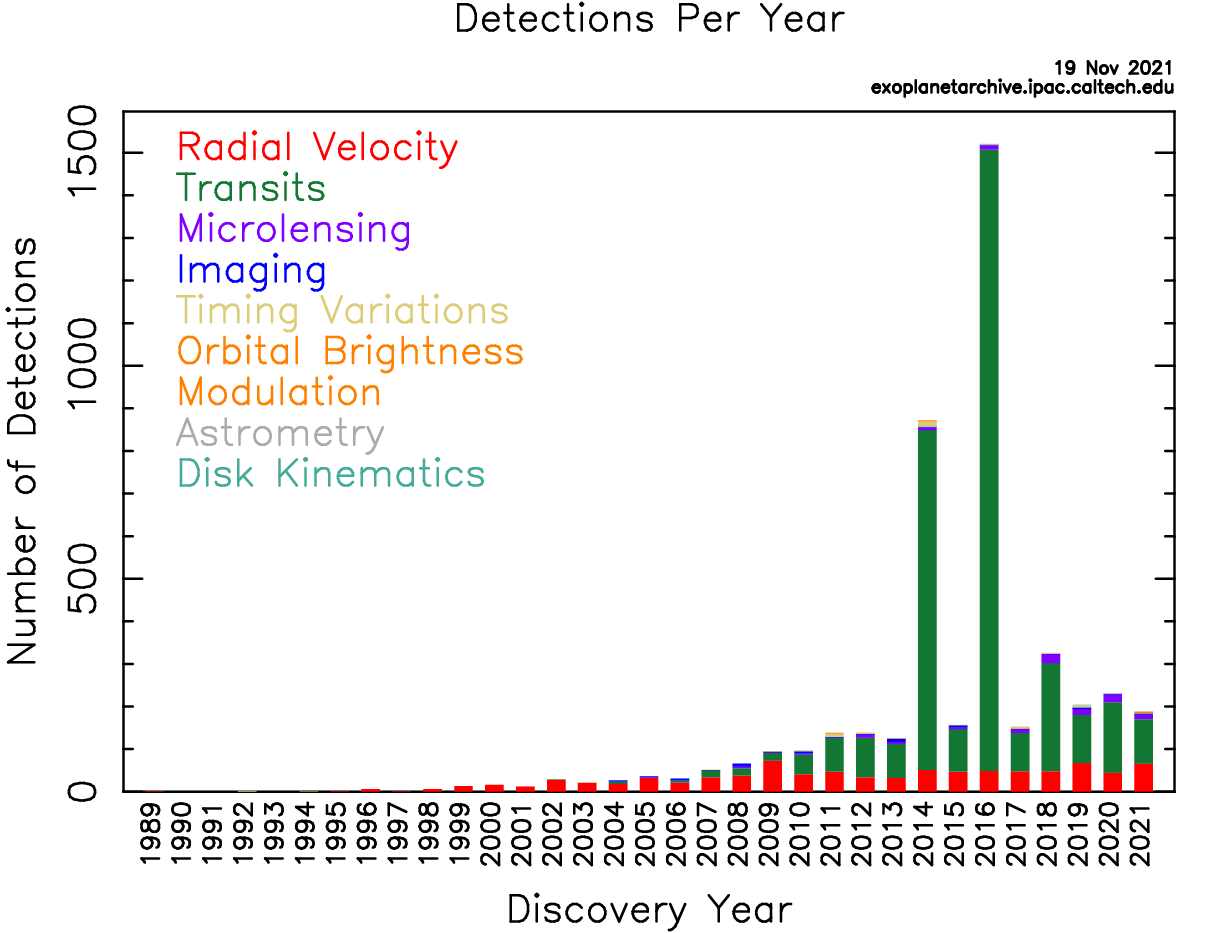
\includegraphics[scale=0.15, angle=0]{../pictures/exo_dischist.png}
    \caption*{\textit{ https://exoplanetarchive.ipac.caltech.edu/}}
\end{figure}
In this report we focus on WASP-44 b, a Jupyter-size planet orbiting around 
a G-type star, located in the constellation of Cetus.
Among the numerous available reports on the planet.

\section{Instruments}

Bla bla



\section{Theoretical recap}

A brief overview of the transit method

maybe a comment on the bias of the transit method (big planets, close to the star)




\subsection{Bla bla}

\section{Data analysis}

\subsection{Inferring mass and radius}

Using PARAM: what we have, what we get

\subsection{Limb darkening correction}

\subsection{Bias and flat field correction}

\subsection{Extracting the light curve}


\section{Conclusions}

Bla bla

\end{document}